\documentclass[twoside]{book}

% Packages required by doxygen
\usepackage{fixltx2e}
\usepackage{calc}
\usepackage{doxygen}
\usepackage[export]{adjustbox} % also loads graphicx
\usepackage{graphicx}
\usepackage[utf8]{inputenc}
\usepackage{makeidx}
\usepackage{multicol}
\usepackage{multirow}
\PassOptionsToPackage{warn}{textcomp}
\usepackage{textcomp}
\usepackage[nointegrals]{wasysym}
\usepackage[table]{xcolor}

% Font selection
\usepackage[T1]{fontenc}
\usepackage[scaled=.90]{helvet}
\usepackage{courier}
\usepackage{amssymb}
\usepackage{sectsty}
\renewcommand{\familydefault}{\sfdefault}
\allsectionsfont{%
  \fontseries{bc}\selectfont%
  \color{darkgray}%
}
\renewcommand{\DoxyLabelFont}{%
  \fontseries{bc}\selectfont%
  \color{darkgray}%
}
\newcommand{\+}{\discretionary{\mbox{\scriptsize$\hookleftarrow$}}{}{}}

% Page & text layout
\usepackage{geometry}
\geometry{%
  a4paper,%
  top=2.5cm,%
  bottom=2.5cm,%
  left=2.5cm,%
  right=2.5cm%
}
\tolerance=750
\hfuzz=15pt
\hbadness=750
\setlength{\emergencystretch}{15pt}
\setlength{\parindent}{0cm}
\setlength{\parskip}{0.2cm}
\makeatletter
\renewcommand{\paragraph}{%
  \@startsection{paragraph}{4}{0ex}{-1.0ex}{1.0ex}{%
    \normalfont\normalsize\bfseries\SS@parafont%
  }%
}
\renewcommand{\subparagraph}{%
  \@startsection{subparagraph}{5}{0ex}{-1.0ex}{1.0ex}{%
    \normalfont\normalsize\bfseries\SS@subparafont%
  }%
}
\makeatother

% Headers & footers
\usepackage{fancyhdr}
\pagestyle{fancyplain}
\fancyhead[LE]{\fancyplain{}{\bfseries\thepage}}
\fancyhead[CE]{\fancyplain{}{}}
\fancyhead[RE]{\fancyplain{}{\bfseries\leftmark}}
\fancyhead[LO]{\fancyplain{}{\bfseries\rightmark}}
\fancyhead[CO]{\fancyplain{}{}}
\fancyhead[RO]{\fancyplain{}{\bfseries\thepage}}
\fancyfoot[LE]{\fancyplain{}{}}
\fancyfoot[CE]{\fancyplain{}{}}
\fancyfoot[RE]{\fancyplain{}{\bfseries\scriptsize Generated on Wed May 20 2015 05\+:59\+:24 for My Project by Doxygen }}
\fancyfoot[LO]{\fancyplain{}{\bfseries\scriptsize Generated on Wed May 20 2015 05\+:59\+:24 for My Project by Doxygen }}
\fancyfoot[CO]{\fancyplain{}{}}
\fancyfoot[RO]{\fancyplain{}{}}
\renewcommand{\footrulewidth}{0.4pt}
\renewcommand{\chaptermark}[1]{%
  \markboth{#1}{}%
}
\renewcommand{\sectionmark}[1]{%
  \markright{\thesection\ #1}%
}

% Indices & bibliography
\usepackage{natbib}
\usepackage[titles]{tocloft}
\setcounter{tocdepth}{3}
\setcounter{secnumdepth}{5}
\makeindex

% Hyperlinks (required, but should be loaded last)
\usepackage{ifpdf}
\ifpdf
  \usepackage[pdftex,pagebackref=true]{hyperref}
\else
  \usepackage[ps2pdf,pagebackref=true]{hyperref}
\fi
\hypersetup{%
  colorlinks=true,%
  linkcolor=blue,%
  citecolor=blue,%
  unicode%
}

% Custom commands
\newcommand{\clearemptydoublepage}{%
  \newpage{\pagestyle{empty}\cleardoublepage}%
}


%===== C O N T E N T S =====

\begin{document}

% Titlepage & ToC
\hypersetup{pageanchor=false,
             bookmarks=true,
             bookmarksnumbered=true,
             pdfencoding=unicode
            }
\pagenumbering{roman}
\begin{titlepage}
\vspace*{7cm}
\begin{center}%
{\Large My Project }\\
\vspace*{1cm}
{\large Generated by Doxygen 1.8.9.1}\\
\vspace*{0.5cm}
{\small Wed May 20 2015 05:59:24}\\
\end{center}
\end{titlepage}
\clearemptydoublepage
\tableofcontents
\clearemptydoublepage
\pagenumbering{arabic}
\hypersetup{pageanchor=true}

%--- Begin generated contents ---
\chapter{Hierarchical Index}
\section{Class Hierarchy}
This inheritance list is sorted roughly, but not completely, alphabetically\+:\begin{DoxyCompactList}
\item \contentsline{section}{entrada\+Historial}{\pageref{classentradaHistorial}}{}
\item \contentsline{section}{Fecha}{\pageref{classFecha}}{}
\item \contentsline{section}{Nego}{\pageref{classNego}}{}
\item \contentsline{section}{Oficina}{\pageref{classOficina}}{}
\item \contentsline{section}{Owner}{\pageref{classOwner}}{}
\item \contentsline{section}{Peticion}{\pageref{classPeticion}}{}
\item Q\+Dialog\begin{DoxyCompactList}
\item \contentsline{section}{dialog\+Informe}{\pageref{classdialogInforme}}{}
\item \contentsline{section}{dialog\+Login}{\pageref{classdialogLogin}}{}
\item \contentsline{section}{dialog\+Nego}{\pageref{classdialogNego}}{}
\item \contentsline{section}{dialog\+Oficinas}{\pageref{classdialogOficinas}}{}
\item \contentsline{section}{dialog\+Owner}{\pageref{classdialogOwner}}{}
\item \contentsline{section}{dialog\+Peticiones}{\pageref{classdialogPeticiones}}{}
\end{DoxyCompactList}
\item Q\+Main\+Window\begin{DoxyCompactList}
\item \contentsline{section}{main\+Window}{\pageref{classmainWindow}}{}
\end{DoxyCompactList}
\item \contentsline{section}{rank}{\pageref{structrank}}{}
\item \contentsline{section}{pel\+:\+:Vector$<$ T $>$}{\pageref{classpel_1_1Vector}}{}
\item \contentsline{section}{pel\+:\+:Vector$<$ entrada\+Historial $>$}{\pageref{classpel_1_1Vector}}{}
\item \contentsline{section}{pel\+:\+:Vector$<$ Oficina $>$}{\pageref{classpel_1_1Vector}}{}
\item \contentsline{section}{pel\+:\+:Vector$<$ Owner $>$}{\pageref{classpel_1_1Vector}}{}
\item \contentsline{section}{pel\+:\+:Vector$<$ Peticion $>$}{\pageref{classpel_1_1Vector}}{}
\item \contentsline{section}{pel\+:\+:Vector$<$ std\+:\+:shared\+\_\+ptr$<$ Nego $>$ $>$}{\pageref{classpel_1_1Vector}}{}
\end{DoxyCompactList}

\chapter{Class Index}
\section{Class List}
Here are the classes, structs, unions and interfaces with brief descriptions\+:\begin{DoxyCompactList}
\item\contentsline{section}{\hyperlink{classdialogInforme}{dialog\+Informe} }{\pageref{classdialogInforme}}{}
\item\contentsline{section}{\hyperlink{classdialogLogin}{dialog\+Login} \\*Dialogo de Usuarios }{\pageref{classdialogLogin}}{}
\item\contentsline{section}{\hyperlink{classdialogNego}{dialog\+Nego} \\*Dialogo de Negos }{\pageref{classdialogNego}}{}
\item\contentsline{section}{\hyperlink{classdialogOficinas}{dialog\+Oficinas} \\*Dialogo de Oficinas }{\pageref{classdialogOficinas}}{}
\item\contentsline{section}{\hyperlink{classdialogOwner}{dialog\+Owner} \\*Dialogo de Owners }{\pageref{classdialogOwner}}{}
\item\contentsline{section}{\hyperlink{classdialogPeticiones}{dialog\+Peticiones} \\*The \hyperlink{classdialogPeticiones}{dialog\+Peticiones} class }{\pageref{classdialogPeticiones}}{}
\item\contentsline{section}{\hyperlink{classentradaHistorial}{entrada\+Historial} }{\pageref{classentradaHistorial}}{}
\item\contentsline{section}{\hyperlink{classFecha}{Fecha} \\*Clase \hyperlink{classFecha}{Fecha} }{\pageref{classFecha}}{}
\item\contentsline{section}{\hyperlink{classmainWindow}{main\+Window} \\*Ventana Principal }{\pageref{classmainWindow}}{}
\item\contentsline{section}{\hyperlink{classNego}{Nego} \\*Clase \hyperlink{classNego}{Nego} Un \hyperlink{classNego}{Nego} es un vuelo concreto. Contiente Origen y Destino, unas Plazas, una \hyperlink{classFecha}{Fecha} concreta y pertenece a un único \hyperlink{classOwner}{Owner} }{\pageref{classNego}}{}
\item\contentsline{section}{\hyperlink{classOficina}{Oficina} }{\pageref{classOficina}}{}
\item\contentsline{section}{\hyperlink{classOwner}{Owner} \\*Clase \hyperlink{classOwner}{Owner} }{\pageref{classOwner}}{}
\item\contentsline{section}{\hyperlink{classPeticion}{Peticion} \\*The \hyperlink{classPeticion}{Peticion} class }{\pageref{classPeticion}}{}
\item\contentsline{section}{\hyperlink{structrank}{rank} }{\pageref{structrank}}{}
\item\contentsline{section}{\hyperlink{classpel_1_1Vector}{pel\+::\+Vector$<$ T $>$} }{\pageref{classpel_1_1Vector}}{}
\end{DoxyCompactList}

\chapter{Class Documentation}
\hypertarget{structBF__ctx}{}\section{B\+F\+\_\+ctx Struct Reference}
\label{structBF__ctx}\index{B\+F\+\_\+ctx@{B\+F\+\_\+ctx}}
\subsection*{Public Attributes}
\begin{DoxyCompactItemize}
\item 
\hypertarget{structBF__ctx_ae16879b199664e199cacb4fe5d43d94b}{}B\+F\+\_\+word {\bfseries S} \mbox{[}4\mbox{]}\mbox{[}0x100\mbox{]}\label{structBF__ctx_ae16879b199664e199cacb4fe5d43d94b}

\item 
\hypertarget{structBF__ctx_a54b05caa5443c19de34d210ec7b13120}{}B\+F\+\_\+key {\bfseries P}\label{structBF__ctx_a54b05caa5443c19de34d210ec7b13120}

\end{DoxyCompactItemize}


The documentation for this struct was generated from the following file\+:\begin{DoxyCompactItemize}
\item 
bcrypt.\+cpp\end{DoxyCompactItemize}

\hypertarget{classdiagOwner}{}\section{diag\+Owner Class Reference}
\label{classdiagOwner}\index{diag\+Owner@{diag\+Owner}}


The \hyperlink{classdiagOwner}{diag\+Owner} class.  




{\ttfamily \#include $<$diagowner.\+hpp$>$}



Inheritance diagram for diag\+Owner\+:
\nopagebreak
\begin{figure}[H]
\begin{center}
\leavevmode
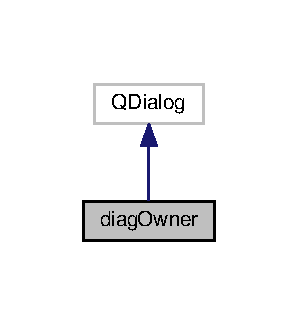
\includegraphics[width=143pt]{classdiagOwner__inherit__graph}
\end{center}
\end{figure}


Collaboration diagram for diag\+Owner\+:
\nopagebreak
\begin{figure}[H]
\begin{center}
\leavevmode
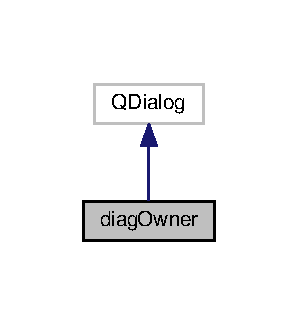
\includegraphics[width=143pt]{classdiagOwner__coll__graph}
\end{center}
\end{figure}
\subsection*{Public Member Functions}
\begin{DoxyCompactItemize}
\item 
\hyperlink{classdiagOwner_a97c3f1ea7838f58881ca683c673d3fd9}{diag\+Owner} (Q\+Widget $\ast$parent=0)
\begin{DoxyCompactList}\small\item\em \hyperlink{classdiagOwner}{diag\+Owner} \end{DoxyCompactList}\item 
\hypertarget{classdiagOwner_ada2fa9627fd5ee15d304e36225c61e49}{}\hyperlink{classdiagOwner_ada2fa9627fd5ee15d304e36225c61e49}{$\sim$diag\+Owner} ()\label{classdiagOwner_ada2fa9627fd5ee15d304e36225c61e49}

\begin{DoxyCompactList}\small\item\em \hyperlink{classdiagOwner_ada2fa9627fd5ee15d304e36225c61e49}{diag\+Owner\+::$\sim$diag\+Owner} \end{DoxyCompactList}\item 
void \hyperlink{classdiagOwner_a959bea0fcf0af99211559fa8eac779c6}{set\+Ow} (std\+::vector$<$ \hyperlink{classOwner}{Owner} $>$ \&own)
\begin{DoxyCompactList}\small\item\em set\+Ow \end{DoxyCompactList}\item 
void \hyperlink{classdiagOwner_aafa9885bca20002ea2a6ad44f1ebb1be}{set\+Row} (int index)
\begin{DoxyCompactList}\small\item\em set\+Row \end{DoxyCompactList}\end{DoxyCompactItemize}


\subsection{Detailed Description}
The \hyperlink{classdiagOwner}{diag\+Owner} class. 

\subsection{Constructor \& Destructor Documentation}
\hypertarget{classdiagOwner_a97c3f1ea7838f58881ca683c673d3fd9}{}\index{diag\+Owner@{diag\+Owner}!diag\+Owner@{diag\+Owner}}
\index{diag\+Owner@{diag\+Owner}!diag\+Owner@{diag\+Owner}}
\subsubsection[{diag\+Owner}]{\setlength{\rightskip}{0pt plus 5cm}diag\+Owner\+::diag\+Owner (
\begin{DoxyParamCaption}
\item[{Q\+Widget $\ast$}]{parent = {\ttfamily 0}}
\end{DoxyParamCaption}
)\hspace{0.3cm}{\ttfamily [explicit]}}\label{classdiagOwner_a97c3f1ea7838f58881ca683c673d3fd9}


\hyperlink{classdiagOwner}{diag\+Owner} 

\hyperlink{classdiagOwner_a97c3f1ea7838f58881ca683c673d3fd9}{diag\+Owner\+::diag\+Owner}


\begin{DoxyParams}{Parameters}
{\em parent} & \\
\hline
{\em parent} & ui \\
\hline
\end{DoxyParams}


\subsection{Member Function Documentation}
\hypertarget{classdiagOwner_a959bea0fcf0af99211559fa8eac779c6}{}\index{diag\+Owner@{diag\+Owner}!set\+Ow@{set\+Ow}}
\index{set\+Ow@{set\+Ow}!diag\+Owner@{diag\+Owner}}
\subsubsection[{set\+Ow}]{\setlength{\rightskip}{0pt plus 5cm}void diag\+Owner\+::set\+Ow (
\begin{DoxyParamCaption}
\item[{std\+::vector$<$ {\bf Owner} $>$ \&}]{own}
\end{DoxyParamCaption}
)}\label{classdiagOwner_a959bea0fcf0af99211559fa8eac779c6}


set\+Ow 

\hyperlink{classdiagOwner_a959bea0fcf0af99211559fa8eac779c6}{diag\+Owner\+::set\+Ow}


\begin{DoxyParams}{Parameters}
{\em own} & \\
\hline
\end{DoxyParams}
\hypertarget{classdiagOwner_aafa9885bca20002ea2a6ad44f1ebb1be}{}\index{diag\+Owner@{diag\+Owner}!set\+Row@{set\+Row}}
\index{set\+Row@{set\+Row}!diag\+Owner@{diag\+Owner}}
\subsubsection[{set\+Row}]{\setlength{\rightskip}{0pt plus 5cm}void diag\+Owner\+::set\+Row (
\begin{DoxyParamCaption}
\item[{int}]{index}
\end{DoxyParamCaption}
)}\label{classdiagOwner_aafa9885bca20002ea2a6ad44f1ebb1be}


set\+Row 

\hyperlink{classdiagOwner_aafa9885bca20002ea2a6ad44f1ebb1be}{diag\+Owner\+::set\+Row}


\begin{DoxyParams}{Parameters}
{\em index} & \\
\hline
\end{DoxyParams}


The documentation for this class was generated from the following files\+:\begin{DoxyCompactItemize}
\item 
diagowner.\+hpp\item 
diagowner.\+cpp\end{DoxyCompactItemize}

\hypertarget{classDialogNego}{}\section{Dialog\+Nego Class Reference}
\label{classDialogNego}\index{Dialog\+Nego@{Dialog\+Nego}}


The \hyperlink{classDialogNego}{Dialog\+Nego} class.  




{\ttfamily \#include $<$dialognego.\+hpp$>$}



Inheritance diagram for Dialog\+Nego\+:
\nopagebreak
\begin{figure}[H]
\begin{center}
\leavevmode
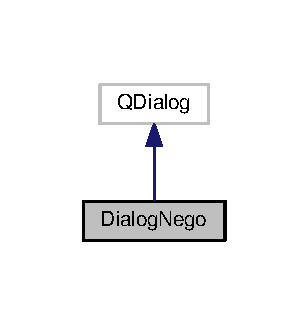
\includegraphics[width=148pt]{classDialogNego__inherit__graph}
\end{center}
\end{figure}


Collaboration diagram for Dialog\+Nego\+:
\nopagebreak
\begin{figure}[H]
\begin{center}
\leavevmode
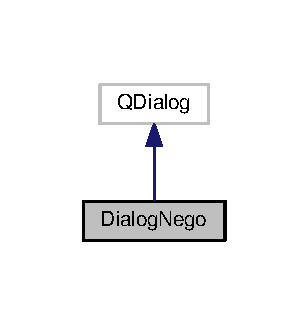
\includegraphics[width=148pt]{classDialogNego__coll__graph}
\end{center}
\end{figure}
\subsection*{Public Member Functions}
\begin{DoxyCompactItemize}
\item 
\hyperlink{classDialogNego_af8f2a27c7f024fd866eda40b6840ec04}{Dialog\+Nego} (Q\+Widget $\ast$parent=0)
\begin{DoxyCompactList}\small\item\em \hyperlink{classDialogNego}{Dialog\+Nego}. \end{DoxyCompactList}\item 
\hypertarget{classDialogNego_a674a6a1fd42ba00bd85279430f7e4d94}{}\hyperlink{classDialogNego_a674a6a1fd42ba00bd85279430f7e4d94}{$\sim$\+Dialog\+Nego} ()\label{classDialogNego_a674a6a1fd42ba00bd85279430f7e4d94}

\begin{DoxyCompactList}\small\item\em \hyperlink{classDialogNego_a674a6a1fd42ba00bd85279430f7e4d94}{Dialog\+Nego\+::$\sim$\+Dialog\+Nego}. \end{DoxyCompactList}\item 
void \hyperlink{classDialogNego_a559476945fd30cbe286824404eb76c89}{set\+Ne} (std\+::vector$<$ std\+::shared\+\_\+ptr$<$ \hyperlink{classNego}{Nego} $>$$>$ \&neg)
\begin{DoxyCompactList}\small\item\em set\+Ne \end{DoxyCompactList}\item 
void \hyperlink{classDialogNego_ab395a294d1be0e12b3ecf2a38742f713}{set\+Ow} (std\+::vector$<$ \hyperlink{classOwner}{Owner} $>$ \&own)
\begin{DoxyCompactList}\small\item\em set\+Ow \end{DoxyCompactList}\item 
void \hyperlink{classDialogNego_a5e976097b3dbecc695ed5153bc09d18a}{cargar} ()
\begin{DoxyCompactList}\small\item\em cargar \end{DoxyCompactList}\item 
void \hyperlink{classDialogNego_ad98c2abab579325665c3b2f615aeb08c}{set\+Rows} (int mod\+Row\+Owner, int mod\+Row\+Nego)
\begin{DoxyCompactList}\small\item\em set\+Rows \end{DoxyCompactList}\end{DoxyCompactItemize}


\subsection{Detailed Description}
The \hyperlink{classDialogNego}{Dialog\+Nego} class. 

\subsection{Constructor \& Destructor Documentation}
\hypertarget{classDialogNego_af8f2a27c7f024fd866eda40b6840ec04}{}\index{Dialog\+Nego@{Dialog\+Nego}!Dialog\+Nego@{Dialog\+Nego}}
\index{Dialog\+Nego@{Dialog\+Nego}!Dialog\+Nego@{Dialog\+Nego}}
\subsubsection[{Dialog\+Nego}]{\setlength{\rightskip}{0pt plus 5cm}Dialog\+Nego\+::\+Dialog\+Nego (
\begin{DoxyParamCaption}
\item[{Q\+Widget $\ast$}]{parent = {\ttfamily 0}}
\end{DoxyParamCaption}
)\hspace{0.3cm}{\ttfamily [explicit]}}\label{classDialogNego_af8f2a27c7f024fd866eda40b6840ec04}


\hyperlink{classDialogNego}{Dialog\+Nego}. 

\hyperlink{classDialogNego_af8f2a27c7f024fd866eda40b6840ec04}{Dialog\+Nego\+::\+Dialog\+Nego}.


\begin{DoxyParams}{Parameters}
{\em parent} & \\
\hline
{\em parent} & ui \\
\hline
\end{DoxyParams}


\subsection{Member Function Documentation}
\hypertarget{classDialogNego_a5e976097b3dbecc695ed5153bc09d18a}{}\index{Dialog\+Nego@{Dialog\+Nego}!cargar@{cargar}}
\index{cargar@{cargar}!Dialog\+Nego@{Dialog\+Nego}}
\subsubsection[{cargar}]{\setlength{\rightskip}{0pt plus 5cm}void Dialog\+Nego\+::cargar (
\begin{DoxyParamCaption}
{}
\end{DoxyParamCaption}
)}\label{classDialogNego_a5e976097b3dbecc695ed5153bc09d18a}


cargar 

\hyperlink{classDialogNego_a5e976097b3dbecc695ed5153bc09d18a}{Dialog\+Nego\+::cargar}. \hypertarget{classDialogNego_a559476945fd30cbe286824404eb76c89}{}\index{Dialog\+Nego@{Dialog\+Nego}!set\+Ne@{set\+Ne}}
\index{set\+Ne@{set\+Ne}!Dialog\+Nego@{Dialog\+Nego}}
\subsubsection[{set\+Ne}]{\setlength{\rightskip}{0pt plus 5cm}void Dialog\+Nego\+::set\+Ne (
\begin{DoxyParamCaption}
\item[{std\+::vector$<$ std\+::shared\+\_\+ptr$<$ {\bf Nego} $>$$>$ \&}]{neg}
\end{DoxyParamCaption}
)}\label{classDialogNego_a559476945fd30cbe286824404eb76c89}


set\+Ne 

\hyperlink{classDialogNego_a559476945fd30cbe286824404eb76c89}{Dialog\+Nego\+::set\+Ne}.


\begin{DoxyParams}{Parameters}
{\em neg} & \\
\hline
\end{DoxyParams}
\hypertarget{classDialogNego_ab395a294d1be0e12b3ecf2a38742f713}{}\index{Dialog\+Nego@{Dialog\+Nego}!set\+Ow@{set\+Ow}}
\index{set\+Ow@{set\+Ow}!Dialog\+Nego@{Dialog\+Nego}}
\subsubsection[{set\+Ow}]{\setlength{\rightskip}{0pt plus 5cm}void Dialog\+Nego\+::set\+Ow (
\begin{DoxyParamCaption}
\item[{std\+::vector$<$ {\bf Owner} $>$ \&}]{own}
\end{DoxyParamCaption}
)}\label{classDialogNego_ab395a294d1be0e12b3ecf2a38742f713}


set\+Ow 

\hyperlink{classDialogNego_ab395a294d1be0e12b3ecf2a38742f713}{Dialog\+Nego\+::set\+Ow}.


\begin{DoxyParams}{Parameters}
{\em own} & \\
\hline
\end{DoxyParams}
\hypertarget{classDialogNego_ad98c2abab579325665c3b2f615aeb08c}{}\index{Dialog\+Nego@{Dialog\+Nego}!set\+Rows@{set\+Rows}}
\index{set\+Rows@{set\+Rows}!Dialog\+Nego@{Dialog\+Nego}}
\subsubsection[{set\+Rows}]{\setlength{\rightskip}{0pt plus 5cm}void Dialog\+Nego\+::set\+Rows (
\begin{DoxyParamCaption}
\item[{int}]{mod\+Row\+Owner, }
\item[{int}]{mod\+Row\+Nego}
\end{DoxyParamCaption}
)}\label{classDialogNego_ad98c2abab579325665c3b2f615aeb08c}


set\+Rows 

\hyperlink{classDialogNego_ad98c2abab579325665c3b2f615aeb08c}{Dialog\+Nego\+::set\+Rows}.


\begin{DoxyParams}{Parameters}
{\em mod\+Row\+Owner} & \\
\hline
{\em mod\+Row\+Nego} & \\
\hline
\end{DoxyParams}


The documentation for this class was generated from the following files\+:\begin{DoxyCompactItemize}
\item 
dialognego.\+hpp\item 
dialognego.\+cpp\end{DoxyCompactItemize}

\hypertarget{classDialogOficina}{}\section{Dialog\+Oficina Class Reference}
\label{classDialogOficina}\index{Dialog\+Oficina@{Dialog\+Oficina}}


Inheritance diagram for Dialog\+Oficina\+:
\nopagebreak
\begin{figure}[H]
\begin{center}
\leavevmode
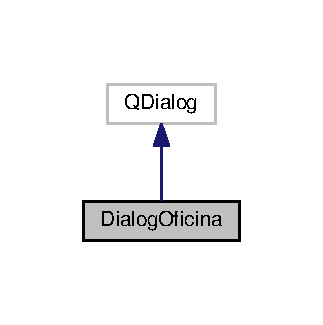
\includegraphics[width=155pt]{classDialogOficina__inherit__graph}
\end{center}
\end{figure}


Collaboration diagram for Dialog\+Oficina\+:
\nopagebreak
\begin{figure}[H]
\begin{center}
\leavevmode
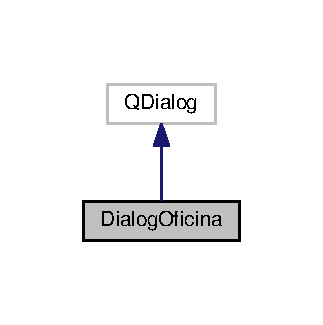
\includegraphics[width=155pt]{classDialogOficina__coll__graph}
\end{center}
\end{figure}
\subsection*{Public Member Functions}
\begin{DoxyCompactItemize}
\item 
\hypertarget{classDialogOficina_a3ad9c07c53db92bc142f57a8ff2f882d}{}{\bfseries Dialog\+Oficina} (Q\+Widget $\ast$parent=0)\label{classDialogOficina_a3ad9c07c53db92bc142f57a8ff2f882d}

\item 
\hypertarget{classDialogOficina_a007a57b696f328e8ecf439e60cd2e034}{}void {\bfseries set\+Of} (std\+::vector$<$ \hyperlink{classOficina}{Oficina} $>$ \&ofi)\label{classDialogOficina_a007a57b696f328e8ecf439e60cd2e034}

\item 
\hypertarget{classDialogOficina_a91bf5c089d49dd8c3f3cfd14e3ff0a59}{}void {\bfseries set\+Ow} (std\+::vector$<$ \hyperlink{classOwner}{Owner} $>$ \&own)\label{classDialogOficina_a91bf5c089d49dd8c3f3cfd14e3ff0a59}

\item 
\hypertarget{classDialogOficina_a0e28e820df54cad3652e7d36a2fd01bc}{}void {\bfseries cargar} ()\label{classDialogOficina_a0e28e820df54cad3652e7d36a2fd01bc}

\end{DoxyCompactItemize}


The documentation for this class was generated from the following files\+:\begin{DoxyCompactItemize}
\item 
dialogoficina.\+h\item 
dialogoficina.\+cpp\end{DoxyCompactItemize}

\hypertarget{classDialogOficinas}{}\section{Dialog\+Oficinas Class Reference}
\label{classDialogOficinas}\index{Dialog\+Oficinas@{Dialog\+Oficinas}}


Inheritance diagram for Dialog\+Oficinas\+:
\nopagebreak
\begin{figure}[H]
\begin{center}
\leavevmode
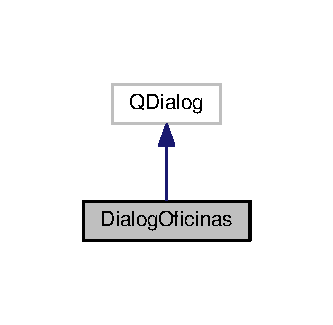
\includegraphics[width=160pt]{classDialogOficinas__inherit__graph}
\end{center}
\end{figure}


Collaboration diagram for Dialog\+Oficinas\+:
\nopagebreak
\begin{figure}[H]
\begin{center}
\leavevmode
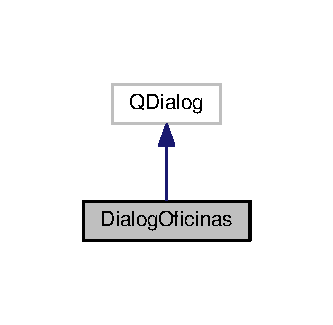
\includegraphics[width=160pt]{classDialogOficinas__coll__graph}
\end{center}
\end{figure}
\subsection*{Public Member Functions}
\begin{DoxyCompactItemize}
\item 
\hypertarget{classDialogOficinas_ad6a35128c2eb7c8f3e38db464d451142}{}{\bfseries Dialog\+Oficinas} (Q\+Widget $\ast$parent=0)\label{classDialogOficinas_ad6a35128c2eb7c8f3e38db464d451142}

\item 
\hypertarget{classDialogOficinas_a848379b90b4b090dda20f398eb2aecaf}{}void {\bfseries set\+Of} (std\+::vector$<$ \hyperlink{classOficina}{Oficina} $>$ \&ofc)\label{classDialogOficinas_a848379b90b4b090dda20f398eb2aecaf}

\item 
\hypertarget{classDialogOficinas_a0bbcb3a5ad14e2886ec3db535c9f7c86}{}void {\bfseries set\+Ow} (std\+::vector$<$ \hyperlink{classOwner}{Owner} $>$ \&own)\label{classDialogOficinas_a0bbcb3a5ad14e2886ec3db535c9f7c86}

\item 
\hypertarget{classDialogOficinas_a35c31c78feea1e2f73fc01ad3c90c09d}{}void {\bfseries set\+Pe} (std\+::vector$<$ \hyperlink{classPeticion}{Peticion} $>$ \&pet)\label{classDialogOficinas_a35c31c78feea1e2f73fc01ad3c90c09d}

\item 
\hypertarget{classDialogOficinas_a640b675822fb98a9fe2e20fb4f5043c7}{}void {\bfseries set\+Rows} (int mod\+Row\+Owner, int mod\+Row\+Oficina)\label{classDialogOficinas_a640b675822fb98a9fe2e20fb4f5043c7}

\item 
\hypertarget{classDialogOficinas_a8d83fdb7fc51dca3676b0d7f0ade6144}{}void {\bfseries cargar} ()\label{classDialogOficinas_a8d83fdb7fc51dca3676b0d7f0ade6144}

\end{DoxyCompactItemize}


The documentation for this class was generated from the following files\+:\begin{DoxyCompactItemize}
\item 
dialog\+Oficinas.\+hpp\item 
dialog\+Oficinas.\+cpp\end{DoxyCompactItemize}

\hypertarget{classDialogPeticiones}{}\section{Dialog\+Peticiones Class Reference}
\label{classDialogPeticiones}\index{Dialog\+Peticiones@{Dialog\+Peticiones}}


The \hyperlink{classDialogPeticiones}{Dialog\+Peticiones} class.  




{\ttfamily \#include $<$dialogpeticiones.\+hpp$>$}



Inheritance diagram for Dialog\+Peticiones\+:
\nopagebreak
\begin{figure}[H]
\begin{center}
\leavevmode
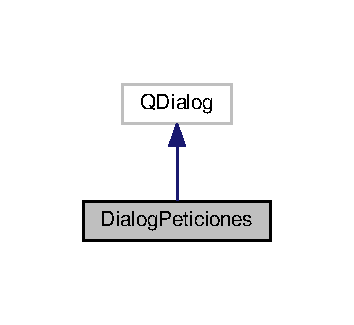
\includegraphics[width=170pt]{classDialogPeticiones__inherit__graph}
\end{center}
\end{figure}


Collaboration diagram for Dialog\+Peticiones\+:
\nopagebreak
\begin{figure}[H]
\begin{center}
\leavevmode
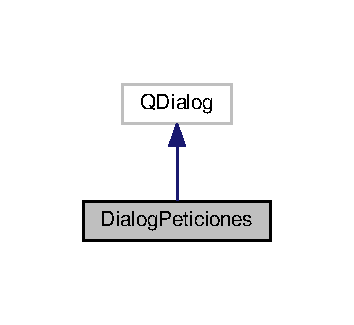
\includegraphics[width=170pt]{classDialogPeticiones__coll__graph}
\end{center}
\end{figure}
\subsection*{Public Member Functions}
\begin{DoxyCompactItemize}
\item 
\hyperlink{classDialogPeticiones_aa21bc875975e468ceab548f6fa23e4c5}{Dialog\+Peticiones} (Q\+Widget $\ast$parent=0)
\begin{DoxyCompactList}\small\item\em \hyperlink{classDialogPeticiones}{Dialog\+Peticiones}. \end{DoxyCompactList}\item 
\hypertarget{classDialogPeticiones_ae8b45e18bccff1ec86e525b817bba912}{}\hyperlink{classDialogPeticiones_ae8b45e18bccff1ec86e525b817bba912}{$\sim$\+Dialog\+Peticiones} ()\label{classDialogPeticiones_ae8b45e18bccff1ec86e525b817bba912}

\begin{DoxyCompactList}\small\item\em \hyperlink{classDialogPeticiones_ae8b45e18bccff1ec86e525b817bba912}{Dialog\+Peticiones\+::$\sim$\+Dialog\+Peticiones}. \end{DoxyCompactList}\item 
void \hyperlink{classDialogPeticiones_a7084e851f919b8fdb9e91110cda77c7f}{set\+Ow} (std\+::vector$<$ \hyperlink{classOwner}{Owner} $>$ \&own)
\begin{DoxyCompactList}\small\item\em set\+Ow \end{DoxyCompactList}\item 
void \hyperlink{classDialogPeticiones_a5c7ea55482f49534c0ee5ed671253f24}{set\+Pe} (std\+::vector$<$ \hyperlink{classPeticion}{Peticion} $>$ \&pet)
\begin{DoxyCompactList}\small\item\em set\+Pe \end{DoxyCompactList}\item 
\hypertarget{classDialogPeticiones_a537bb011119f744329fd347588c5ce02}{}void \hyperlink{classDialogPeticiones_a537bb011119f744329fd347588c5ce02}{set\+Of} (std\+::vector$<$ \hyperlink{classOficina}{Oficina} $>$ \&of)\label{classDialogPeticiones_a537bb011119f744329fd347588c5ce02}

\begin{DoxyCompactList}\small\item\em cargar \end{DoxyCompactList}\item 
\hypertarget{classDialogPeticiones_abe4b4d742a1b4bb462827de496d7b5fe}{}void {\bfseries set\+Ne} (std\+::vector$<$ std\+::shared\+\_\+ptr$<$ \hyperlink{classNego}{Nego} $>$$>$ \&ne)\label{classDialogPeticiones_abe4b4d742a1b4bb462827de496d7b5fe}

\item 
\hypertarget{classDialogPeticiones_a715b3453eb8b3b8f0d558b53fcc18fdf}{}void \hyperlink{classDialogPeticiones_a715b3453eb8b3b8f0d558b53fcc18fdf}{cargar} ()\label{classDialogPeticiones_a715b3453eb8b3b8f0d558b53fcc18fdf}

\begin{DoxyCompactList}\small\item\em \hyperlink{classDialogPeticiones_a715b3453eb8b3b8f0d558b53fcc18fdf}{Dialog\+Peticiones\+::cargar}. \end{DoxyCompactList}\end{DoxyCompactItemize}


\subsection{Detailed Description}
The \hyperlink{classDialogPeticiones}{Dialog\+Peticiones} class. 

\subsection{Constructor \& Destructor Documentation}
\hypertarget{classDialogPeticiones_aa21bc875975e468ceab548f6fa23e4c5}{}\index{Dialog\+Peticiones@{Dialog\+Peticiones}!Dialog\+Peticiones@{Dialog\+Peticiones}}
\index{Dialog\+Peticiones@{Dialog\+Peticiones}!Dialog\+Peticiones@{Dialog\+Peticiones}}
\subsubsection[{Dialog\+Peticiones}]{\setlength{\rightskip}{0pt plus 5cm}Dialog\+Peticiones\+::\+Dialog\+Peticiones (
\begin{DoxyParamCaption}
\item[{Q\+Widget $\ast$}]{parent = {\ttfamily 0}}
\end{DoxyParamCaption}
)\hspace{0.3cm}{\ttfamily [explicit]}}\label{classDialogPeticiones_aa21bc875975e468ceab548f6fa23e4c5}


\hyperlink{classDialogPeticiones}{Dialog\+Peticiones}. 

ui


\begin{DoxyParams}{Parameters}
{\em parent} & \\
\hline
\end{DoxyParams}


\subsection{Member Function Documentation}
\hypertarget{classDialogPeticiones_a7084e851f919b8fdb9e91110cda77c7f}{}\index{Dialog\+Peticiones@{Dialog\+Peticiones}!set\+Ow@{set\+Ow}}
\index{set\+Ow@{set\+Ow}!Dialog\+Peticiones@{Dialog\+Peticiones}}
\subsubsection[{set\+Ow}]{\setlength{\rightskip}{0pt plus 5cm}void Dialog\+Peticiones\+::set\+Ow (
\begin{DoxyParamCaption}
\item[{std\+::vector$<$ {\bf Owner} $>$ \&}]{own}
\end{DoxyParamCaption}
)}\label{classDialogPeticiones_a7084e851f919b8fdb9e91110cda77c7f}


set\+Ow 

\hyperlink{classDialogPeticiones_a7084e851f919b8fdb9e91110cda77c7f}{Dialog\+Peticiones\+::set\+Ow}.


\begin{DoxyParams}{Parameters}
{\em own} & \\
\hline
\end{DoxyParams}
\hypertarget{classDialogPeticiones_a5c7ea55482f49534c0ee5ed671253f24}{}\index{Dialog\+Peticiones@{Dialog\+Peticiones}!set\+Pe@{set\+Pe}}
\index{set\+Pe@{set\+Pe}!Dialog\+Peticiones@{Dialog\+Peticiones}}
\subsubsection[{set\+Pe}]{\setlength{\rightskip}{0pt plus 5cm}void Dialog\+Peticiones\+::set\+Pe (
\begin{DoxyParamCaption}
\item[{std\+::vector$<$ {\bf Peticion} $>$ \&}]{pet}
\end{DoxyParamCaption}
)}\label{classDialogPeticiones_a5c7ea55482f49534c0ee5ed671253f24}


set\+Pe 

\hyperlink{classDialogPeticiones_a5c7ea55482f49534c0ee5ed671253f24}{Dialog\+Peticiones\+::set\+Pe}.


\begin{DoxyParams}{Parameters}
{\em pet} & \\
\hline
\end{DoxyParams}


The documentation for this class was generated from the following files\+:\begin{DoxyCompactItemize}
\item 
dialogpeticiones.\+hpp\item 
dialogpeticiones.\+cpp\end{DoxyCompactItemize}

\hypertarget{classFecha}{}\section{Fecha Class Reference}
\label{classFecha}\index{Fecha@{Fecha}}


The \hyperlink{classFecha}{Fecha} class.  




{\ttfamily \#include $<$fecha.\+hpp$>$}

\subsection*{Public Member Functions}
\begin{DoxyCompactItemize}
\item 
\hyperlink{classFecha_a5fbc6564d9c48e73cf8d27568a2a7fc5}{Fecha} ()
\begin{DoxyCompactList}\small\item\em \hyperlink{classFecha}{Fecha}. \end{DoxyCompactList}\item 
\hyperlink{classFecha_ac4e53e6fcbb50c3619cfc60e1a5de016}{Fecha} (std\+::size\+\_\+t dia, std\+::size\+\_\+t mes, int anio)
\begin{DoxyCompactList}\small\item\em \hyperlink{classFecha}{Fecha}. \end{DoxyCompactList}\item 
\hypertarget{classFecha_ae34f2ebe1ac7f3a78eefb68e8d1c8b86}{}\hyperlink{classFecha_ae34f2ebe1ac7f3a78eefb68e8d1c8b86}{$\sim$\+Fecha} ()\label{classFecha_ae34f2ebe1ac7f3a78eefb68e8d1c8b86}

\begin{DoxyCompactList}\small\item\em \hyperlink{classFecha_ae34f2ebe1ac7f3a78eefb68e8d1c8b86}{Fecha\+::$\sim$\+Fecha}. \end{DoxyCompactList}\item 
void \hyperlink{classFecha_a3040cb959b0b779c262805460d9786bb}{set\+Fecha} (std\+::size\+\_\+t dia, std\+::size\+\_\+t mes, int anio)
\begin{DoxyCompactList}\small\item\em set\+Fecha \end{DoxyCompactList}\item 
void \hyperlink{classFecha_a19af0818e81aa8d74b60fdfca7aabb04}{set\+Dia} (std\+::size\+\_\+t dia)
\begin{DoxyCompactList}\small\item\em set\+Dia \end{DoxyCompactList}\item 
void \hyperlink{classFecha_a0167b058fedd612cd2c29c3d932d0741}{set\+Mes} (std\+::size\+\_\+t mes)
\begin{DoxyCompactList}\small\item\em set\+Mes \end{DoxyCompactList}\item 
void \hyperlink{classFecha_a3cfbea8834e7a23023f11c3d069838f0}{set\+Anio} (int anio)
\begin{DoxyCompactList}\small\item\em set\+Anio \end{DoxyCompactList}\item 
std\+::size\+\_\+t \hyperlink{classFecha_a1a2191fb9b522845f249f5f1af233f58}{get\+Dia} ()
\begin{DoxyCompactList}\small\item\em get\+Dia \end{DoxyCompactList}\item 
std\+::size\+\_\+t \hyperlink{classFecha_adab1b3eed2b3e81ccf7bc78c456635ce}{get\+Mes} ()
\begin{DoxyCompactList}\small\item\em get\+Mes \end{DoxyCompactList}\item 
int \hyperlink{classFecha_a89ebafe74bc6e5f53ad688dce1d3fc26}{get\+Anio} ()
\begin{DoxyCompactList}\small\item\em get\+Anio \end{DoxyCompactList}\item 
{\footnotesize template$<$class Archive $>$ }\\void \hyperlink{classFecha_a8e2b7a6977d7d6354647af025808f750}{serialize} (Archive \&archive)
\begin{DoxyCompactList}\small\item\em serialize \end{DoxyCompactList}\end{DoxyCompactItemize}


\subsection{Detailed Description}
The \hyperlink{classFecha}{Fecha} class. 

\subsection{Constructor \& Destructor Documentation}
\hypertarget{classFecha_a5fbc6564d9c48e73cf8d27568a2a7fc5}{}\index{Fecha@{Fecha}!Fecha@{Fecha}}
\index{Fecha@{Fecha}!Fecha@{Fecha}}
\subsubsection[{Fecha}]{\setlength{\rightskip}{0pt plus 5cm}Fecha\+::\+Fecha (
\begin{DoxyParamCaption}
{}
\end{DoxyParamCaption}
)}\label{classFecha_a5fbc6564d9c48e73cf8d27568a2a7fc5}


\hyperlink{classFecha}{Fecha}. 

\hyperlink{classFecha_a5fbc6564d9c48e73cf8d27568a2a7fc5}{Fecha\+::\+Fecha}. \hypertarget{classFecha_ac4e53e6fcbb50c3619cfc60e1a5de016}{}\index{Fecha@{Fecha}!Fecha@{Fecha}}
\index{Fecha@{Fecha}!Fecha@{Fecha}}
\subsubsection[{Fecha}]{\setlength{\rightskip}{0pt plus 5cm}Fecha\+::\+Fecha (
\begin{DoxyParamCaption}
\item[{std\+::size\+\_\+t}]{dia, }
\item[{std\+::size\+\_\+t}]{mes, }
\item[{int}]{anio}
\end{DoxyParamCaption}
)}\label{classFecha_ac4e53e6fcbb50c3619cfc60e1a5de016}


\hyperlink{classFecha}{Fecha}. 


\begin{DoxyParams}{Parameters}
{\em dia} & \\
\hline
{\em mes} & \\
\hline
{\em anio} & \\
\hline
\end{DoxyParams}


\subsection{Member Function Documentation}
\hypertarget{classFecha_a89ebafe74bc6e5f53ad688dce1d3fc26}{}\index{Fecha@{Fecha}!get\+Anio@{get\+Anio}}
\index{get\+Anio@{get\+Anio}!Fecha@{Fecha}}
\subsubsection[{get\+Anio}]{\setlength{\rightskip}{0pt plus 5cm}int Fecha\+::get\+Anio (
\begin{DoxyParamCaption}
{}
\end{DoxyParamCaption}
)}\label{classFecha_a89ebafe74bc6e5f53ad688dce1d3fc26}


get\+Anio 

\hyperlink{classFecha_a89ebafe74bc6e5f53ad688dce1d3fc26}{Fecha\+::get\+Anio}.

\begin{DoxyReturn}{Returns}

\end{DoxyReturn}
\hypertarget{classFecha_a1a2191fb9b522845f249f5f1af233f58}{}\index{Fecha@{Fecha}!get\+Dia@{get\+Dia}}
\index{get\+Dia@{get\+Dia}!Fecha@{Fecha}}
\subsubsection[{get\+Dia}]{\setlength{\rightskip}{0pt plus 5cm}size\+\_\+t Fecha\+::get\+Dia (
\begin{DoxyParamCaption}
{}
\end{DoxyParamCaption}
)}\label{classFecha_a1a2191fb9b522845f249f5f1af233f58}


get\+Dia 

\hyperlink{classFecha_a1a2191fb9b522845f249f5f1af233f58}{Fecha\+::get\+Dia}.

\begin{DoxyReturn}{Returns}

\end{DoxyReturn}
\hypertarget{classFecha_adab1b3eed2b3e81ccf7bc78c456635ce}{}\index{Fecha@{Fecha}!get\+Mes@{get\+Mes}}
\index{get\+Mes@{get\+Mes}!Fecha@{Fecha}}
\subsubsection[{get\+Mes}]{\setlength{\rightskip}{0pt plus 5cm}size\+\_\+t Fecha\+::get\+Mes (
\begin{DoxyParamCaption}
{}
\end{DoxyParamCaption}
)}\label{classFecha_adab1b3eed2b3e81ccf7bc78c456635ce}


get\+Mes 

\hyperlink{classFecha_adab1b3eed2b3e81ccf7bc78c456635ce}{Fecha\+::get\+Mes}.

\begin{DoxyReturn}{Returns}

\end{DoxyReturn}
\hypertarget{classFecha_a8e2b7a6977d7d6354647af025808f750}{}\index{Fecha@{Fecha}!serialize@{serialize}}
\index{serialize@{serialize}!Fecha@{Fecha}}
\subsubsection[{serialize}]{\setlength{\rightskip}{0pt plus 5cm}template$<$class Archive $>$ void Fecha\+::serialize (
\begin{DoxyParamCaption}
\item[{Archive \&}]{archive}
\end{DoxyParamCaption}
)\hspace{0.3cm}{\ttfamily [inline]}}\label{classFecha_a8e2b7a6977d7d6354647af025808f750}


serialize 


\begin{DoxyParams}{Parameters}
{\em archive} & \\
\hline
\end{DoxyParams}
archive

cereal\+::make\+\_\+nvp\hypertarget{classFecha_a3cfbea8834e7a23023f11c3d069838f0}{}\index{Fecha@{Fecha}!set\+Anio@{set\+Anio}}
\index{set\+Anio@{set\+Anio}!Fecha@{Fecha}}
\subsubsection[{set\+Anio}]{\setlength{\rightskip}{0pt plus 5cm}void Fecha\+::set\+Anio (
\begin{DoxyParamCaption}
\item[{int}]{anio}
\end{DoxyParamCaption}
)}\label{classFecha_a3cfbea8834e7a23023f11c3d069838f0}


set\+Anio 

\hyperlink{classFecha_a3cfbea8834e7a23023f11c3d069838f0}{Fecha\+::set\+Anio}.


\begin{DoxyParams}{Parameters}
{\em anio} & \\
\hline
\end{DoxyParams}
\hypertarget{classFecha_a19af0818e81aa8d74b60fdfca7aabb04}{}\index{Fecha@{Fecha}!set\+Dia@{set\+Dia}}
\index{set\+Dia@{set\+Dia}!Fecha@{Fecha}}
\subsubsection[{set\+Dia}]{\setlength{\rightskip}{0pt plus 5cm}void Fecha\+::set\+Dia (
\begin{DoxyParamCaption}
\item[{std\+::size\+\_\+t}]{dia}
\end{DoxyParamCaption}
)}\label{classFecha_a19af0818e81aa8d74b60fdfca7aabb04}


set\+Dia 

\hyperlink{classFecha_a19af0818e81aa8d74b60fdfca7aabb04}{Fecha\+::set\+Dia}.


\begin{DoxyParams}{Parameters}
{\em dia} & set\+Dia \\
\hline
{\em dia} & \\
\hline
{\em dia} & \\
\hline
\end{DoxyParams}
\hypertarget{classFecha_a3040cb959b0b779c262805460d9786bb}{}\index{Fecha@{Fecha}!set\+Fecha@{set\+Fecha}}
\index{set\+Fecha@{set\+Fecha}!Fecha@{Fecha}}
\subsubsection[{set\+Fecha}]{\setlength{\rightskip}{0pt plus 5cm}void Fecha\+::set\+Fecha (
\begin{DoxyParamCaption}
\item[{std\+::size\+\_\+t}]{dia, }
\item[{std\+::size\+\_\+t}]{mes, }
\item[{int}]{anio}
\end{DoxyParamCaption}
)}\label{classFecha_a3040cb959b0b779c262805460d9786bb}


set\+Fecha 

\hyperlink{classFecha_a3040cb959b0b779c262805460d9786bb}{Fecha\+::set\+Fecha}.


\begin{DoxyParams}{Parameters}
{\em dia} & \\
\hline
{\em mes} & \\
\hline
{\em anio} & \\
\hline
\end{DoxyParams}
\hypertarget{classFecha_a0167b058fedd612cd2c29c3d932d0741}{}\index{Fecha@{Fecha}!set\+Mes@{set\+Mes}}
\index{set\+Mes@{set\+Mes}!Fecha@{Fecha}}
\subsubsection[{set\+Mes}]{\setlength{\rightskip}{0pt plus 5cm}void Fecha\+::set\+Mes (
\begin{DoxyParamCaption}
\item[{std\+::size\+\_\+t}]{mes}
\end{DoxyParamCaption}
)}\label{classFecha_a0167b058fedd612cd2c29c3d932d0741}


set\+Mes 

\hyperlink{classFecha_a0167b058fedd612cd2c29c3d932d0741}{Fecha\+::set\+Mes}.


\begin{DoxyParams}{Parameters}
{\em mes} & \\
\hline
\end{DoxyParams}


The documentation for this class was generated from the following files\+:\begin{DoxyCompactItemize}
\item 
fecha.\+hpp\item 
fecha.\+cpp\end{DoxyCompactItemize}

\hypertarget{classLogin}{}\section{Login Class Reference}
\label{classLogin}\index{Login@{Login}}


The \hyperlink{classLogin}{Login} class.  




{\ttfamily \#include $<$login.\+hpp$>$}



Inheritance diagram for Login\+:
\nopagebreak
\begin{figure}[H]
\begin{center}
\leavevmode
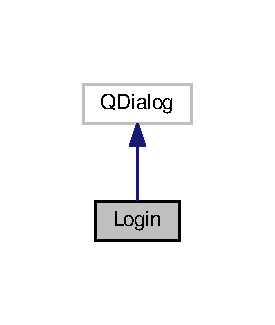
\includegraphics[width=132pt]{classLogin__inherit__graph}
\end{center}
\end{figure}


Collaboration diagram for Login\+:
\nopagebreak
\begin{figure}[H]
\begin{center}
\leavevmode
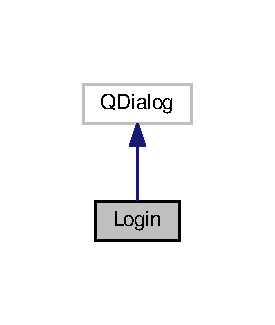
\includegraphics[width=132pt]{classLogin__coll__graph}
\end{center}
\end{figure}
\subsection*{Signals}
\begin{DoxyCompactItemize}
\item 
\hypertarget{classLogin_ab103305ffe0bcdc06392da0934639ef6}{}void \hyperlink{classLogin_ab103305ffe0bcdc06392da0934639ef6}{cambio\+De\+Usuario} (std\+::string)\label{classLogin_ab103305ffe0bcdc06392da0934639ef6}

\begin{DoxyCompactList}\small\item\em cambio\+De\+Usuario \end{DoxyCompactList}\end{DoxyCompactItemize}
\subsection*{Public Member Functions}
\begin{DoxyCompactItemize}
\item 
\hyperlink{classLogin_a021ebcfd29b2a30e3f5c5bbb36589381}{Login} (Q\+Widget $\ast$parent=0)
\begin{DoxyCompactList}\small\item\em \hyperlink{classLogin}{Login}. \end{DoxyCompactList}\item 
void \hyperlink{classLogin_a0d877d8c08f419c62e5eaecabe6fa3de}{set\+Estado} (int estado)
\begin{DoxyCompactList}\small\item\em set\+Estado \end{DoxyCompactList}\item 
\hypertarget{classLogin_a659bc7233ec12c79b9fa523c1734fbbc}{}\hyperlink{classLogin_a659bc7233ec12c79b9fa523c1734fbbc}{$\sim$\+Login} ()\label{classLogin_a659bc7233ec12c79b9fa523c1734fbbc}

\begin{DoxyCompactList}\small\item\em \hyperlink{classLogin_a659bc7233ec12c79b9fa523c1734fbbc}{Login\+::$\sim$\+Login}. \end{DoxyCompactList}\end{DoxyCompactItemize}


\subsection{Detailed Description}
The \hyperlink{classLogin}{Login} class. 

\subsection{Constructor \& Destructor Documentation}
\hypertarget{classLogin_a021ebcfd29b2a30e3f5c5bbb36589381}{}\index{Login@{Login}!Login@{Login}}
\index{Login@{Login}!Login@{Login}}
\subsubsection[{Login}]{\setlength{\rightskip}{0pt plus 5cm}Login\+::\+Login (
\begin{DoxyParamCaption}
\item[{Q\+Widget $\ast$}]{parent = {\ttfamily 0}}
\end{DoxyParamCaption}
)\hspace{0.3cm}{\ttfamily [explicit]}}\label{classLogin_a021ebcfd29b2a30e3f5c5bbb36589381}


\hyperlink{classLogin}{Login}. 

\hyperlink{classLogin_a021ebcfd29b2a30e3f5c5bbb36589381}{Login\+::\+Login}.


\begin{DoxyParams}{Parameters}
{\em parent} & \\
\hline
\end{DoxyParams}


\subsection{Member Function Documentation}
\hypertarget{classLogin_a0d877d8c08f419c62e5eaecabe6fa3de}{}\index{Login@{Login}!set\+Estado@{set\+Estado}}
\index{set\+Estado@{set\+Estado}!Login@{Login}}
\subsubsection[{set\+Estado}]{\setlength{\rightskip}{0pt plus 5cm}void Login\+::set\+Estado (
\begin{DoxyParamCaption}
\item[{int}]{estado}
\end{DoxyParamCaption}
)}\label{classLogin_a0d877d8c08f419c62e5eaecabe6fa3de}


set\+Estado 

\hyperlink{classLogin_a0d877d8c08f419c62e5eaecabe6fa3de}{Login\+::set\+Estado}.


\begin{DoxyParams}{Parameters}
{\em estado} & \\
\hline
\end{DoxyParams}


The documentation for this class was generated from the following files\+:\begin{DoxyCompactItemize}
\item 
login.\+hpp\item 
login.\+cpp\end{DoxyCompactItemize}

\hypertarget{classMainWindow}{}\section{Main\+Window Class Reference}
\label{classMainWindow}\index{Main\+Window@{Main\+Window}}


The \hyperlink{classMainWindow}{Main\+Window} class.  




{\ttfamily \#include $<$mainwindow.\+hpp$>$}



Inheritance diagram for Main\+Window\+:
\nopagebreak
\begin{figure}[H]
\begin{center}
\leavevmode
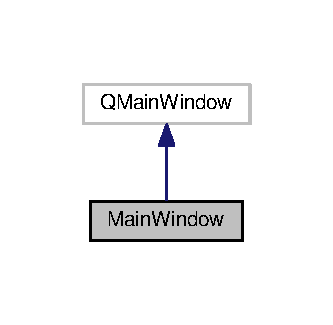
\includegraphics[width=160pt]{classMainWindow__inherit__graph}
\end{center}
\end{figure}


Collaboration diagram for Main\+Window\+:
\nopagebreak
\begin{figure}[H]
\begin{center}
\leavevmode
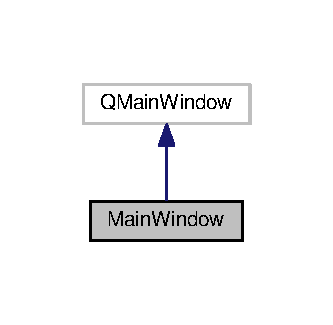
\includegraphics[width=160pt]{classMainWindow__coll__graph}
\end{center}
\end{figure}
\subsection*{Public Member Functions}
\begin{DoxyCompactItemize}
\item 
\hyperlink{classMainWindow_a8b244be8b7b7db1b08de2a2acb9409db}{Main\+Window} (Q\+Widget $\ast$parent=0)
\begin{DoxyCompactList}\small\item\em \hyperlink{classMainWindow}{Main\+Window}. \end{DoxyCompactList}\item 
\hypertarget{classMainWindow_ae98d00a93bc118200eeef9f9bba1dba7}{}\hyperlink{classMainWindow_ae98d00a93bc118200eeef9f9bba1dba7}{$\sim$\+Main\+Window} ()\label{classMainWindow_ae98d00a93bc118200eeef9f9bba1dba7}

\begin{DoxyCompactList}\small\item\em \hyperlink{classMainWindow_ae98d00a93bc118200eeef9f9bba1dba7}{Main\+Window\+::$\sim$\+Main\+Window}. \end{DoxyCompactList}\end{DoxyCompactItemize}


\subsection{Detailed Description}
The \hyperlink{classMainWindow}{Main\+Window} class. 

\subsection{Constructor \& Destructor Documentation}
\hypertarget{classMainWindow_a8b244be8b7b7db1b08de2a2acb9409db}{}\index{Main\+Window@{Main\+Window}!Main\+Window@{Main\+Window}}
\index{Main\+Window@{Main\+Window}!Main\+Window@{Main\+Window}}
\subsubsection[{Main\+Window}]{\setlength{\rightskip}{0pt plus 5cm}Main\+Window\+::\+Main\+Window (
\begin{DoxyParamCaption}
\item[{Q\+Widget $\ast$}]{parent = {\ttfamily 0}}
\end{DoxyParamCaption}
)\hspace{0.3cm}{\ttfamily [explicit]}}\label{classMainWindow_a8b244be8b7b7db1b08de2a2acb9409db}


\hyperlink{classMainWindow}{Main\+Window}. 

\hyperlink{classMainWindow_a8b244be8b7b7db1b08de2a2acb9409db}{Main\+Window\+::\+Main\+Window}.


\begin{DoxyParams}{Parameters}
{\em parent} & \\
\hline
\end{DoxyParams}


The documentation for this class was generated from the following files\+:\begin{DoxyCompactItemize}
\item 
mainwindow.\+hpp\item 
mainwindow.\+cpp\end{DoxyCompactItemize}

\hypertarget{classNego}{}\section{Nego Class Reference}
\label{classNego}\index{Nego@{Nego}}


The \hyperlink{classNego}{Nego} class.  




{\ttfamily \#include $<$nego.\+hpp$>$}

\subsection*{Public Member Functions}
\begin{DoxyCompactItemize}
\item 
\hyperlink{classNego_af997efc08cdc4e0fc654e6294ac4b08b}{Nego} ()
\begin{DoxyCompactList}\small\item\em \hyperlink{classNego}{Nego}. \end{DoxyCompactList}\item 
\hyperlink{classNego_a612bceb68453277f47491aa2cdaf0963}{Nego} (std\+::string origen, std\+::string destino, int numero\+Plazas, \hyperlink{classFecha}{Fecha} fecha)
\begin{DoxyCompactList}\small\item\em \hyperlink{classNego}{Nego}. \end{DoxyCompactList}\item 
\hypertarget{classNego_af7be4e019e1aa8aaae080e9900574c74}{}\hyperlink{classNego_af7be4e019e1aa8aaae080e9900574c74}{$\sim$\+Nego} ()\label{classNego_af7be4e019e1aa8aaae080e9900574c74}

\begin{DoxyCompactList}\small\item\em \hyperlink{classNego_af7be4e019e1aa8aaae080e9900574c74}{Nego\+::$\sim$\+Nego}. \end{DoxyCompactList}\item 
void \hyperlink{classNego_a886d652e1dd9f66c387978dbbcbf6aec}{set\+Nego} (std\+::string origen, std\+::string destino, int numero\+Plazas, \hyperlink{classFecha}{Fecha} fecha)
\begin{DoxyCompactList}\small\item\em set\+Nego \end{DoxyCompactList}\item 
void \hyperlink{classNego_ab9a55ac4fb4834dbede2806dbbcb62bb}{set\+Origen} (std\+::string origen)
\begin{DoxyCompactList}\small\item\em set\+Origen \end{DoxyCompactList}\item 
void \hyperlink{classNego_a037842afd947e4f33de78ecb4ce0485c}{set\+Destino} (std\+::string destino)
\begin{DoxyCompactList}\small\item\em set\+Destino \end{DoxyCompactList}\item 
void \hyperlink{classNego_ad3b026b1faf221046acb58ee10906ec8}{set\+Numero\+Plazas} (int numero\+Plazas)
\begin{DoxyCompactList}\small\item\em set\+Numero\+Plazas \end{DoxyCompactList}\item 
void \hyperlink{classNego_a8fd1c05283f046daab60ed330bac1795}{set\+Fecha} (\hyperlink{classFecha}{Fecha} fecha)
\begin{DoxyCompactList}\small\item\em set\+Fecha \end{DoxyCompactList}\item 
std\+::string \hyperlink{classNego_a6be2088a392ae71ae25ff281e8432cc3}{get\+Origen} ()
\begin{DoxyCompactList}\small\item\em get\+Origen \end{DoxyCompactList}\item 
std\+::string \hyperlink{classNego_ade01b1e886a2b8e68152338a0ffd1240}{get\+Destino} ()
\begin{DoxyCompactList}\small\item\em get\+Destino \end{DoxyCompactList}\item 
int \hyperlink{classNego_a28cd95d6e56112d813e2128d553cdae7}{get\+Numero\+Plazas} ()
\begin{DoxyCompactList}\small\item\em get\+Numero\+Plazas \end{DoxyCompactList}\item 
\hyperlink{classFecha}{Fecha} \hyperlink{classNego_a83559824f47d518d3bb70d260262d676}{get\+Fecha} ()
\begin{DoxyCompactList}\small\item\em get\+Fecha \end{DoxyCompactList}\item 
{\footnotesize template$<$class Archive $>$ }\\void \hyperlink{classNego_af2aa46474903fc02942fa44d4576fcad}{serialize} (Archive \&archive)
\begin{DoxyCompactList}\small\item\em serialize \end{DoxyCompactList}\end{DoxyCompactItemize}


\subsection{Detailed Description}
The \hyperlink{classNego}{Nego} class. 

\subsection{Constructor \& Destructor Documentation}
\hypertarget{classNego_af997efc08cdc4e0fc654e6294ac4b08b}{}\index{Nego@{Nego}!Nego@{Nego}}
\index{Nego@{Nego}!Nego@{Nego}}
\subsubsection[{Nego}]{\setlength{\rightskip}{0pt plus 5cm}Nego\+::\+Nego (
\begin{DoxyParamCaption}
{}
\end{DoxyParamCaption}
)}\label{classNego_af997efc08cdc4e0fc654e6294ac4b08b}


\hyperlink{classNego}{Nego}. 

\hyperlink{classNego_af997efc08cdc4e0fc654e6294ac4b08b}{Nego\+::\+Nego}. \hypertarget{classNego_a612bceb68453277f47491aa2cdaf0963}{}\index{Nego@{Nego}!Nego@{Nego}}
\index{Nego@{Nego}!Nego@{Nego}}
\subsubsection[{Nego}]{\setlength{\rightskip}{0pt plus 5cm}Nego\+::\+Nego (
\begin{DoxyParamCaption}
\item[{std\+::string}]{origen, }
\item[{std\+::string}]{destino, }
\item[{int}]{numero\+Plazas, }
\item[{{\bf Fecha}}]{fecha}
\end{DoxyParamCaption}
)}\label{classNego_a612bceb68453277f47491aa2cdaf0963}


\hyperlink{classNego}{Nego}. 

\hyperlink{classNego_af997efc08cdc4e0fc654e6294ac4b08b}{Nego\+::\+Nego}.


\begin{DoxyParams}{Parameters}
{\em origen} & \\
\hline
{\em destino} & \\
\hline
{\em numero\+Plazas} & \\
\hline
{\em fecha} & \\
\hline
\end{DoxyParams}


\subsection{Member Function Documentation}
\hypertarget{classNego_ade01b1e886a2b8e68152338a0ffd1240}{}\index{Nego@{Nego}!get\+Destino@{get\+Destino}}
\index{get\+Destino@{get\+Destino}!Nego@{Nego}}
\subsubsection[{get\+Destino}]{\setlength{\rightskip}{0pt plus 5cm}std\+::string Nego\+::get\+Destino (
\begin{DoxyParamCaption}
{}
\end{DoxyParamCaption}
)}\label{classNego_ade01b1e886a2b8e68152338a0ffd1240}


get\+Destino 

\hyperlink{classNego_ade01b1e886a2b8e68152338a0ffd1240}{Nego\+::get\+Destino}.

\begin{DoxyReturn}{Returns}

\end{DoxyReturn}
\hypertarget{classNego_a83559824f47d518d3bb70d260262d676}{}\index{Nego@{Nego}!get\+Fecha@{get\+Fecha}}
\index{get\+Fecha@{get\+Fecha}!Nego@{Nego}}
\subsubsection[{get\+Fecha}]{\setlength{\rightskip}{0pt plus 5cm}{\bf Fecha} Nego\+::get\+Fecha (
\begin{DoxyParamCaption}
{}
\end{DoxyParamCaption}
)}\label{classNego_a83559824f47d518d3bb70d260262d676}


get\+Fecha 

\hyperlink{classNego_a83559824f47d518d3bb70d260262d676}{Nego\+::get\+Fecha}.

\begin{DoxyReturn}{Returns}

\end{DoxyReturn}
\hypertarget{classNego_a28cd95d6e56112d813e2128d553cdae7}{}\index{Nego@{Nego}!get\+Numero\+Plazas@{get\+Numero\+Plazas}}
\index{get\+Numero\+Plazas@{get\+Numero\+Plazas}!Nego@{Nego}}
\subsubsection[{get\+Numero\+Plazas}]{\setlength{\rightskip}{0pt plus 5cm}int Nego\+::get\+Numero\+Plazas (
\begin{DoxyParamCaption}
{}
\end{DoxyParamCaption}
)}\label{classNego_a28cd95d6e56112d813e2128d553cdae7}


get\+Numero\+Plazas 

\hyperlink{classNego_a28cd95d6e56112d813e2128d553cdae7}{Nego\+::get\+Numero\+Plazas}.

\begin{DoxyReturn}{Returns}

\end{DoxyReturn}
\hypertarget{classNego_a6be2088a392ae71ae25ff281e8432cc3}{}\index{Nego@{Nego}!get\+Origen@{get\+Origen}}
\index{get\+Origen@{get\+Origen}!Nego@{Nego}}
\subsubsection[{get\+Origen}]{\setlength{\rightskip}{0pt plus 5cm}std\+::string Nego\+::get\+Origen (
\begin{DoxyParamCaption}
{}
\end{DoxyParamCaption}
)}\label{classNego_a6be2088a392ae71ae25ff281e8432cc3}


get\+Origen 

\hyperlink{classNego_a6be2088a392ae71ae25ff281e8432cc3}{Nego\+::get\+Origen}.

\begin{DoxyReturn}{Returns}

\end{DoxyReturn}
\hypertarget{classNego_af2aa46474903fc02942fa44d4576fcad}{}\index{Nego@{Nego}!serialize@{serialize}}
\index{serialize@{serialize}!Nego@{Nego}}
\subsubsection[{serialize}]{\setlength{\rightskip}{0pt plus 5cm}template$<$class Archive $>$ void Nego\+::serialize (
\begin{DoxyParamCaption}
\item[{Archive \&}]{archive}
\end{DoxyParamCaption}
)\hspace{0.3cm}{\ttfamily [inline]}}\label{classNego_af2aa46474903fc02942fa44d4576fcad}


serialize 


\begin{DoxyParams}{Parameters}
{\em archive} & \\
\hline
\end{DoxyParams}
archive

cereal\+::make\+\_\+nvp

cereal\+::make\+\_\+nvp\hypertarget{classNego_a037842afd947e4f33de78ecb4ce0485c}{}\index{Nego@{Nego}!set\+Destino@{set\+Destino}}
\index{set\+Destino@{set\+Destino}!Nego@{Nego}}
\subsubsection[{set\+Destino}]{\setlength{\rightskip}{0pt plus 5cm}void Nego\+::set\+Destino (
\begin{DoxyParamCaption}
\item[{std\+::string}]{destino}
\end{DoxyParamCaption}
)}\label{classNego_a037842afd947e4f33de78ecb4ce0485c}


set\+Destino 

\hyperlink{classNego_a037842afd947e4f33de78ecb4ce0485c}{Nego\+::set\+Destino}.


\begin{DoxyParams}{Parameters}
{\em destino} & \\
\hline
\end{DoxyParams}
\hypertarget{classNego_a8fd1c05283f046daab60ed330bac1795}{}\index{Nego@{Nego}!set\+Fecha@{set\+Fecha}}
\index{set\+Fecha@{set\+Fecha}!Nego@{Nego}}
\subsubsection[{set\+Fecha}]{\setlength{\rightskip}{0pt plus 5cm}void Nego\+::set\+Fecha (
\begin{DoxyParamCaption}
\item[{{\bf Fecha}}]{fecha}
\end{DoxyParamCaption}
)}\label{classNego_a8fd1c05283f046daab60ed330bac1795}


set\+Fecha 

\hyperlink{classNego_a8fd1c05283f046daab60ed330bac1795}{Nego\+::set\+Fecha}.


\begin{DoxyParams}{Parameters}
{\em fecha} & \\
\hline
\end{DoxyParams}
\hypertarget{classNego_a886d652e1dd9f66c387978dbbcbf6aec}{}\index{Nego@{Nego}!set\+Nego@{set\+Nego}}
\index{set\+Nego@{set\+Nego}!Nego@{Nego}}
\subsubsection[{set\+Nego}]{\setlength{\rightskip}{0pt plus 5cm}void Nego\+::set\+Nego (
\begin{DoxyParamCaption}
\item[{std\+::string}]{origen, }
\item[{std\+::string}]{destino, }
\item[{int}]{numero\+Plazas, }
\item[{{\bf Fecha}}]{fecha}
\end{DoxyParamCaption}
)}\label{classNego_a886d652e1dd9f66c387978dbbcbf6aec}


set\+Nego 

\hyperlink{classNego_a886d652e1dd9f66c387978dbbcbf6aec}{Nego\+::set\+Nego}.


\begin{DoxyParams}{Parameters}
{\em origen} & \\
\hline
{\em destino} & \\
\hline
{\em numero\+Plazas} & \\
\hline
{\em fecha} & \\
\hline
\end{DoxyParams}
\hypertarget{classNego_ad3b026b1faf221046acb58ee10906ec8}{}\index{Nego@{Nego}!set\+Numero\+Plazas@{set\+Numero\+Plazas}}
\index{set\+Numero\+Plazas@{set\+Numero\+Plazas}!Nego@{Nego}}
\subsubsection[{set\+Numero\+Plazas}]{\setlength{\rightskip}{0pt plus 5cm}void Nego\+::set\+Numero\+Plazas (
\begin{DoxyParamCaption}
\item[{int}]{numero\+Plazas}
\end{DoxyParamCaption}
)}\label{classNego_ad3b026b1faf221046acb58ee10906ec8}


set\+Numero\+Plazas 

\hyperlink{classNego_ad3b026b1faf221046acb58ee10906ec8}{Nego\+::set\+Numero\+Plazas}.


\begin{DoxyParams}{Parameters}
{\em numero\+Plazas} & \\
\hline
\end{DoxyParams}
\hypertarget{classNego_ab9a55ac4fb4834dbede2806dbbcb62bb}{}\index{Nego@{Nego}!set\+Origen@{set\+Origen}}
\index{set\+Origen@{set\+Origen}!Nego@{Nego}}
\subsubsection[{set\+Origen}]{\setlength{\rightskip}{0pt plus 5cm}void Nego\+::set\+Origen (
\begin{DoxyParamCaption}
\item[{std\+::string}]{origen}
\end{DoxyParamCaption}
)}\label{classNego_ab9a55ac4fb4834dbede2806dbbcb62bb}


set\+Origen 

\hyperlink{classNego_ab9a55ac4fb4834dbede2806dbbcb62bb}{Nego\+::set\+Origen}.


\begin{DoxyParams}{Parameters}
{\em origen} & \\
\hline
\end{DoxyParams}


The documentation for this class was generated from the following files\+:\begin{DoxyCompactItemize}
\item 
nego.\+hpp\item 
nego.\+cpp\end{DoxyCompactItemize}

\hypertarget{classOficina}{}\section{Oficina Class Reference}
\label{classOficina}\index{Oficina@{Oficina}}


The \hyperlink{classOficina}{Oficina} class.  




{\ttfamily \#include $<$oficina.\+hpp$>$}

\subsection*{Public Member Functions}
\begin{DoxyCompactItemize}
\item 
\hyperlink{classOficina_adfc639739930fedda32e7790583f2342}{Oficina} ()
\begin{DoxyCompactList}\small\item\em \hyperlink{classOficina}{Oficina}. \end{DoxyCompactList}\item 
\hyperlink{classOficina_a98663f13af9d8679a234e3c68c4ceb36}{Oficina} (std\+::string nombre, std\+::string pais, std\+::string continente)
\begin{DoxyCompactList}\small\item\em \hyperlink{classOficina}{Oficina}. \end{DoxyCompactList}\item 
\hypertarget{classOficina_a34125758ffc92b87f19e21d24cb92c60}{}\hyperlink{classOficina_a34125758ffc92b87f19e21d24cb92c60}{$\sim$\+Oficina} ()\label{classOficina_a34125758ffc92b87f19e21d24cb92c60}

\begin{DoxyCompactList}\small\item\em \hyperlink{classOficina_a34125758ffc92b87f19e21d24cb92c60}{Oficina\+::$\sim$\+Oficina}. \end{DoxyCompactList}\item 
void \hyperlink{classOficina_ae016add6b9338df63c58a850b3503d45}{set\+Nombre} (std\+::string)
\begin{DoxyCompactList}\small\item\em set\+Nombre \end{DoxyCompactList}\item 
void \hyperlink{classOficina_a69be721387f2b3b97b0c6a6326d046e5}{set\+Pais} (std\+::string)
\begin{DoxyCompactList}\small\item\em set\+Pais \end{DoxyCompactList}\item 
void \hyperlink{classOficina_a0b715231faa1dc769fd6006f8136626f}{set\+Continente} (std\+::string)
\begin{DoxyCompactList}\small\item\em set\+Continente \end{DoxyCompactList}\item 
std\+::string \hyperlink{classOficina_ad9ef736810c608638d70fd003db62661}{get\+Nombre} ()
\begin{DoxyCompactList}\small\item\em get\+Nombre \end{DoxyCompactList}\item 
std\+::string \hyperlink{classOficina_aef61125dc2cbbe125b4c027196e9cbb3}{get\+Pais} ()
\begin{DoxyCompactList}\small\item\em get\+Pais \end{DoxyCompactList}\item 
std\+::string \hyperlink{classOficina_a937105d318a0554fe2ce00cd59f35160}{get\+Continente} ()
\begin{DoxyCompactList}\small\item\em get\+Continente \end{DoxyCompactList}\item 
std\+::vector$<$ \hyperlink{classPeticion}{Peticion} $>$ \& \hyperlink{classOficina_ab496b537dfe209239796f7f0832dd1b8}{get\+Peticiones} ()
\begin{DoxyCompactList}\small\item\em get\+Peticiones \end{DoxyCompactList}\item 
{\footnotesize template$<$class Archive $>$ }\\void \hyperlink{classOficina_af600ad5dff1f832387e48f2d88bd2b72}{serialize} (Archive \&archive)
\begin{DoxyCompactList}\small\item\em serialize \end{DoxyCompactList}\end{DoxyCompactItemize}


\subsection{Detailed Description}
The \hyperlink{classOficina}{Oficina} class. 

\subsection{Constructor \& Destructor Documentation}
\hypertarget{classOficina_adfc639739930fedda32e7790583f2342}{}\index{Oficina@{Oficina}!Oficina@{Oficina}}
\index{Oficina@{Oficina}!Oficina@{Oficina}}
\subsubsection[{Oficina}]{\setlength{\rightskip}{0pt plus 5cm}Oficina\+::\+Oficina (
\begin{DoxyParamCaption}
{}
\end{DoxyParamCaption}
)}\label{classOficina_adfc639739930fedda32e7790583f2342}


\hyperlink{classOficina}{Oficina}. 

\hyperlink{classOficina_adfc639739930fedda32e7790583f2342}{Oficina\+::\+Oficina}. \hypertarget{classOficina_a98663f13af9d8679a234e3c68c4ceb36}{}\index{Oficina@{Oficina}!Oficina@{Oficina}}
\index{Oficina@{Oficina}!Oficina@{Oficina}}
\subsubsection[{Oficina}]{\setlength{\rightskip}{0pt plus 5cm}Oficina\+::\+Oficina (
\begin{DoxyParamCaption}
\item[{std\+::string}]{nombre, }
\item[{std\+::string}]{pais, }
\item[{std\+::string}]{continente}
\end{DoxyParamCaption}
)}\label{classOficina_a98663f13af9d8679a234e3c68c4ceb36}


\hyperlink{classOficina}{Oficina}. 

\hyperlink{classOficina_adfc639739930fedda32e7790583f2342}{Oficina\+::\+Oficina}.


\begin{DoxyParams}{Parameters}
{\em nombre} & \\
\hline
{\em pais} & \\
\hline
{\em continente} & \\
\hline
\end{DoxyParams}


\subsection{Member Function Documentation}
\hypertarget{classOficina_a937105d318a0554fe2ce00cd59f35160}{}\index{Oficina@{Oficina}!get\+Continente@{get\+Continente}}
\index{get\+Continente@{get\+Continente}!Oficina@{Oficina}}
\subsubsection[{get\+Continente}]{\setlength{\rightskip}{0pt plus 5cm}std\+::string Oficina\+::get\+Continente (
\begin{DoxyParamCaption}
{}
\end{DoxyParamCaption}
)}\label{classOficina_a937105d318a0554fe2ce00cd59f35160}


get\+Continente 

\hyperlink{classOficina_a937105d318a0554fe2ce00cd59f35160}{Oficina\+::get\+Continente}.

\begin{DoxyReturn}{Returns}

\end{DoxyReturn}
\hypertarget{classOficina_ad9ef736810c608638d70fd003db62661}{}\index{Oficina@{Oficina}!get\+Nombre@{get\+Nombre}}
\index{get\+Nombre@{get\+Nombre}!Oficina@{Oficina}}
\subsubsection[{get\+Nombre}]{\setlength{\rightskip}{0pt plus 5cm}std\+::string Oficina\+::get\+Nombre (
\begin{DoxyParamCaption}
{}
\end{DoxyParamCaption}
)}\label{classOficina_ad9ef736810c608638d70fd003db62661}


get\+Nombre 

\hyperlink{classOficina_ad9ef736810c608638d70fd003db62661}{Oficina\+::get\+Nombre}.

\begin{DoxyReturn}{Returns}

\end{DoxyReturn}
\hypertarget{classOficina_aef61125dc2cbbe125b4c027196e9cbb3}{}\index{Oficina@{Oficina}!get\+Pais@{get\+Pais}}
\index{get\+Pais@{get\+Pais}!Oficina@{Oficina}}
\subsubsection[{get\+Pais}]{\setlength{\rightskip}{0pt plus 5cm}std\+::string Oficina\+::get\+Pais (
\begin{DoxyParamCaption}
{}
\end{DoxyParamCaption}
)}\label{classOficina_aef61125dc2cbbe125b4c027196e9cbb3}


get\+Pais 

\hyperlink{classOficina_aef61125dc2cbbe125b4c027196e9cbb3}{Oficina\+::get\+Pais}.

\begin{DoxyReturn}{Returns}

\end{DoxyReturn}
\hypertarget{classOficina_ab496b537dfe209239796f7f0832dd1b8}{}\index{Oficina@{Oficina}!get\+Peticiones@{get\+Peticiones}}
\index{get\+Peticiones@{get\+Peticiones}!Oficina@{Oficina}}
\subsubsection[{get\+Peticiones}]{\setlength{\rightskip}{0pt plus 5cm}std\+::vector$<$ {\bf Peticion} $>$ \& Oficina\+::get\+Peticiones (
\begin{DoxyParamCaption}
{}
\end{DoxyParamCaption}
)}\label{classOficina_ab496b537dfe209239796f7f0832dd1b8}


get\+Peticiones 

\hyperlink{classOficina_ab496b537dfe209239796f7f0832dd1b8}{Oficina\+::get\+Peticiones}.

\begin{DoxyReturn}{Returns}

\end{DoxyReturn}
\hypertarget{classOficina_af600ad5dff1f832387e48f2d88bd2b72}{}\index{Oficina@{Oficina}!serialize@{serialize}}
\index{serialize@{serialize}!Oficina@{Oficina}}
\subsubsection[{serialize}]{\setlength{\rightskip}{0pt plus 5cm}template$<$class Archive $>$ void Oficina\+::serialize (
\begin{DoxyParamCaption}
\item[{Archive \&}]{archive}
\end{DoxyParamCaption}
)\hspace{0.3cm}{\ttfamily [inline]}}\label{classOficina_af600ad5dff1f832387e48f2d88bd2b72}


serialize 


\begin{DoxyParams}{Parameters}
{\em archive} & \\
\hline
\end{DoxyParams}
archive

cereal\+::make\+\_\+nvp

cereal\+::make\+\_\+nvp\hypertarget{classOficina_a0b715231faa1dc769fd6006f8136626f}{}\index{Oficina@{Oficina}!set\+Continente@{set\+Continente}}
\index{set\+Continente@{set\+Continente}!Oficina@{Oficina}}
\subsubsection[{set\+Continente}]{\setlength{\rightskip}{0pt plus 5cm}void Oficina\+::set\+Continente (
\begin{DoxyParamCaption}
\item[{std\+::string}]{continente}
\end{DoxyParamCaption}
)}\label{classOficina_a0b715231faa1dc769fd6006f8136626f}


set\+Continente 

\hyperlink{classOficina_a0b715231faa1dc769fd6006f8136626f}{Oficina\+::set\+Continente}.


\begin{DoxyParams}{Parameters}
{\em continente} & \\
\hline
\end{DoxyParams}
\hypertarget{classOficina_ae016add6b9338df63c58a850b3503d45}{}\index{Oficina@{Oficina}!set\+Nombre@{set\+Nombre}}
\index{set\+Nombre@{set\+Nombre}!Oficina@{Oficina}}
\subsubsection[{set\+Nombre}]{\setlength{\rightskip}{0pt plus 5cm}void Oficina\+::set\+Nombre (
\begin{DoxyParamCaption}
\item[{std\+::string}]{nombre}
\end{DoxyParamCaption}
)}\label{classOficina_ae016add6b9338df63c58a850b3503d45}


set\+Nombre 

\hyperlink{classOficina_ae016add6b9338df63c58a850b3503d45}{Oficina\+::set\+Nombre}.


\begin{DoxyParams}{Parameters}
{\em nombre} & \\
\hline
\end{DoxyParams}
\hypertarget{classOficina_a69be721387f2b3b97b0c6a6326d046e5}{}\index{Oficina@{Oficina}!set\+Pais@{set\+Pais}}
\index{set\+Pais@{set\+Pais}!Oficina@{Oficina}}
\subsubsection[{set\+Pais}]{\setlength{\rightskip}{0pt plus 5cm}void Oficina\+::set\+Pais (
\begin{DoxyParamCaption}
\item[{std\+::string}]{pais}
\end{DoxyParamCaption}
)}\label{classOficina_a69be721387f2b3b97b0c6a6326d046e5}


set\+Pais 

\hyperlink{classOficina_a69be721387f2b3b97b0c6a6326d046e5}{Oficina\+::set\+Pais}.


\begin{DoxyParams}{Parameters}
{\em pais} & \\
\hline
\end{DoxyParams}


The documentation for this class was generated from the following files\+:\begin{DoxyCompactItemize}
\item 
oficina.\+hpp\item 
oficina.\+cpp\end{DoxyCompactItemize}

\hypertarget{classOwner}{}\section{Owner Class Reference}
\label{classOwner}\index{Owner@{Owner}}


The \hyperlink{classOwner}{Owner} class.  




{\ttfamily \#include $<$owner.\+hpp$>$}

\subsection*{Public Member Functions}
\begin{DoxyCompactItemize}
\item 
\hyperlink{classOwner_ab9186e9839a04fe48baad103cc1d0ddb}{Owner} ()
\begin{DoxyCompactList}\small\item\em \hyperlink{classOwner}{Owner}. \end{DoxyCompactList}\item 
\hyperlink{classOwner_a876e5d2ec5c7f0474ac61ae18256a78d}{Owner} (std\+::string nombre)
\begin{DoxyCompactList}\small\item\em \hyperlink{classOwner}{Owner}. \end{DoxyCompactList}\item 
\hypertarget{classOwner_a1ab2bfec69ca4645de7f113f20e868c3}{}\hyperlink{classOwner_a1ab2bfec69ca4645de7f113f20e868c3}{$\sim$\+Owner} ()\label{classOwner_a1ab2bfec69ca4645de7f113f20e868c3}

\begin{DoxyCompactList}\small\item\em \hyperlink{classOwner_a1ab2bfec69ca4645de7f113f20e868c3}{Owner\+::$\sim$\+Owner}. \end{DoxyCompactList}\item 
void \hyperlink{classOwner_a6b7345e565bfcfde59b1871147765535}{set\+Nombre} (std\+::string)
\begin{DoxyCompactList}\small\item\em set\+Nombre \end{DoxyCompactList}\item 
std\+::string \hyperlink{classOwner_a13cd3eb4f058bfb2ea1d4ba05c61f5b8}{get\+Nombre} ()
\begin{DoxyCompactList}\small\item\em get\+Nombre \end{DoxyCompactList}\item 
std\+::vector$<$ std\+::shared\+\_\+ptr$<$ \hyperlink{classNego}{Nego} $>$ $>$ \& \hyperlink{classOwner_a30db4d5859801773a884c05c9a601d9a}{get\+Negos} ()
\begin{DoxyCompactList}\small\item\em get\+Negos \end{DoxyCompactList}\item 
std\+::vector$<$ \hyperlink{classOficina}{Oficina} $>$ \& \hyperlink{classOwner_a57ccce817249862c941aed8776f28364}{get\+Oficinas} ()
\begin{DoxyCompactList}\small\item\em get\+Oficinas \end{DoxyCompactList}\item 
{\footnotesize template$<$class Archive $>$ }\\void \hyperlink{classOwner_a411a7ce0f140930cec5c45b46319894c}{serialize} (Archive \&archive)
\begin{DoxyCompactList}\small\item\em serialize \end{DoxyCompactList}\end{DoxyCompactItemize}


\subsection{Detailed Description}
The \hyperlink{classOwner}{Owner} class. 

\subsection{Constructor \& Destructor Documentation}
\hypertarget{classOwner_ab9186e9839a04fe48baad103cc1d0ddb}{}\index{Owner@{Owner}!Owner@{Owner}}
\index{Owner@{Owner}!Owner@{Owner}}
\subsubsection[{Owner}]{\setlength{\rightskip}{0pt plus 5cm}Owner\+::\+Owner (
\begin{DoxyParamCaption}
{}
\end{DoxyParamCaption}
)}\label{classOwner_ab9186e9839a04fe48baad103cc1d0ddb}


\hyperlink{classOwner}{Owner}. 

\hyperlink{classOwner_ab9186e9839a04fe48baad103cc1d0ddb}{Owner\+::\+Owner}. \hypertarget{classOwner_a876e5d2ec5c7f0474ac61ae18256a78d}{}\index{Owner@{Owner}!Owner@{Owner}}
\index{Owner@{Owner}!Owner@{Owner}}
\subsubsection[{Owner}]{\setlength{\rightskip}{0pt plus 5cm}Owner\+::\+Owner (
\begin{DoxyParamCaption}
\item[{std\+::string}]{nombre}
\end{DoxyParamCaption}
)\hspace{0.3cm}{\ttfamily [explicit]}}\label{classOwner_a876e5d2ec5c7f0474ac61ae18256a78d}


\hyperlink{classOwner}{Owner}. 

\hyperlink{classOwner_ab9186e9839a04fe48baad103cc1d0ddb}{Owner\+::\+Owner}.


\begin{DoxyParams}{Parameters}
{\em nombre} & \\
\hline
\end{DoxyParams}


\subsection{Member Function Documentation}
\hypertarget{classOwner_a30db4d5859801773a884c05c9a601d9a}{}\index{Owner@{Owner}!get\+Negos@{get\+Negos}}
\index{get\+Negos@{get\+Negos}!Owner@{Owner}}
\subsubsection[{get\+Negos}]{\setlength{\rightskip}{0pt plus 5cm}std\+::vector$<$ std\+::shared\+\_\+ptr$<$ {\bf Nego} $>$ $>$ \& Owner\+::get\+Negos (
\begin{DoxyParamCaption}
{}
\end{DoxyParamCaption}
)}\label{classOwner_a30db4d5859801773a884c05c9a601d9a}


get\+Negos 

\hyperlink{classOwner_a30db4d5859801773a884c05c9a601d9a}{Owner\+::get\+Negos}.

\begin{DoxyReturn}{Returns}

\end{DoxyReturn}
\hypertarget{classOwner_a13cd3eb4f058bfb2ea1d4ba05c61f5b8}{}\index{Owner@{Owner}!get\+Nombre@{get\+Nombre}}
\index{get\+Nombre@{get\+Nombre}!Owner@{Owner}}
\subsubsection[{get\+Nombre}]{\setlength{\rightskip}{0pt plus 5cm}std\+::string Owner\+::get\+Nombre (
\begin{DoxyParamCaption}
{}
\end{DoxyParamCaption}
)}\label{classOwner_a13cd3eb4f058bfb2ea1d4ba05c61f5b8}


get\+Nombre 

\hyperlink{classOwner_a13cd3eb4f058bfb2ea1d4ba05c61f5b8}{Owner\+::get\+Nombre}.

\begin{DoxyReturn}{Returns}

\end{DoxyReturn}
\hypertarget{classOwner_a57ccce817249862c941aed8776f28364}{}\index{Owner@{Owner}!get\+Oficinas@{get\+Oficinas}}
\index{get\+Oficinas@{get\+Oficinas}!Owner@{Owner}}
\subsubsection[{get\+Oficinas}]{\setlength{\rightskip}{0pt plus 5cm}std\+::vector$<$ {\bf Oficina} $>$ \& Owner\+::get\+Oficinas (
\begin{DoxyParamCaption}
{}
\end{DoxyParamCaption}
)}\label{classOwner_a57ccce817249862c941aed8776f28364}


get\+Oficinas 

\hyperlink{classOwner_a57ccce817249862c941aed8776f28364}{Owner\+::get\+Oficinas}.

\begin{DoxyReturn}{Returns}

\end{DoxyReturn}
\hypertarget{classOwner_a411a7ce0f140930cec5c45b46319894c}{}\index{Owner@{Owner}!serialize@{serialize}}
\index{serialize@{serialize}!Owner@{Owner}}
\subsubsection[{serialize}]{\setlength{\rightskip}{0pt plus 5cm}template$<$class Archive $>$ void Owner\+::serialize (
\begin{DoxyParamCaption}
\item[{Archive \&}]{archive}
\end{DoxyParamCaption}
)\hspace{0.3cm}{\ttfamily [inline]}}\label{classOwner_a411a7ce0f140930cec5c45b46319894c}


serialize 


\begin{DoxyParams}{Parameters}
{\em archive} & \\
\hline
\end{DoxyParams}
archive

cereal\+::make\+\_\+nvp\hypertarget{classOwner_a6b7345e565bfcfde59b1871147765535}{}\index{Owner@{Owner}!set\+Nombre@{set\+Nombre}}
\index{set\+Nombre@{set\+Nombre}!Owner@{Owner}}
\subsubsection[{set\+Nombre}]{\setlength{\rightskip}{0pt plus 5cm}void Owner\+::set\+Nombre (
\begin{DoxyParamCaption}
\item[{std\+::string}]{nombre}
\end{DoxyParamCaption}
)}\label{classOwner_a6b7345e565bfcfde59b1871147765535}


set\+Nombre 

\hyperlink{classOwner_a6b7345e565bfcfde59b1871147765535}{Owner\+::set\+Nombre}.


\begin{DoxyParams}{Parameters}
{\em nombre} & \\
\hline
\end{DoxyParams}


The documentation for this class was generated from the following files\+:\begin{DoxyCompactItemize}
\item 
owner.\+hpp\item 
owner.\+cpp\end{DoxyCompactItemize}

\hypertarget{classPeticion}{}\section{Peticion Class Reference}
\label{classPeticion}\index{Peticion@{Peticion}}


The \hyperlink{classPeticion}{Peticion} class.  




{\ttfamily \#include $<$peticion.\+hpp$>$}

\subsection*{Public Member Functions}
\begin{DoxyCompactItemize}
\item 
\hyperlink{classPeticion_a04b4090032ff49bcbf965bdd2af9ae90}{Peticion} ()
\item 
\hypertarget{classPeticion_adca26c8f1c41bc14c69cad5ac7713e3c}{}{\bfseries Peticion} (std\+::size\+\_\+t plazas\+Pedidas)\label{classPeticion_adca26c8f1c41bc14c69cad5ac7713e3c}

\item 
\hypertarget{classPeticion_a75bbeae7cedba0b5c32993f1f3f9c7e1}{}void {\bfseries set\+Plazas\+Pedidas} (std\+::size\+\_\+t plazas\+Pedidas)\label{classPeticion_a75bbeae7cedba0b5c32993f1f3f9c7e1}

\item 
\hypertarget{classPeticion_a58a129027db952f86676a721c7acc6c4}{}std\+::size\+\_\+t {\bfseries get\+Plazas\+Pedidas} ()\label{classPeticion_a58a129027db952f86676a721c7acc6c4}

\end{DoxyCompactItemize}
\subsection*{Public Attributes}
\begin{DoxyCompactItemize}
\item 
\hypertarget{classPeticion_ac38e3db0706f2889ccd473a7af22d4ec}{}std\+::shared\+\_\+ptr$<$ \hyperlink{classNego}{Nego} $>$ {\bfseries neg}\label{classPeticion_ac38e3db0706f2889ccd473a7af22d4ec}

\end{DoxyCompactItemize}


\subsection{Detailed Description}
The \hyperlink{classPeticion}{Peticion} class. 

Copyright 2015 Viaje\+Facil \begin{DoxyAuthor}{Author}
Hugo Ferrando Seage 

David Jimenez 

Serigo Cander las peticiones son elaboradas por todas las partes de este proyecto, es decir, cada acción que se realice va a ser una petición que se quedará guardada en esta clase \char`\"{}peticiones\char`\"{} 
\end{DoxyAuthor}


\subsection{Constructor \& Destructor Documentation}
\hypertarget{classPeticion_a04b4090032ff49bcbf965bdd2af9ae90}{}\index{Peticion@{Peticion}!Peticion@{Peticion}}
\index{Peticion@{Peticion}!Peticion@{Peticion}}
\subsubsection[{Peticion}]{\setlength{\rightskip}{0pt plus 5cm}Peticion\+::\+Peticion (
\begin{DoxyParamCaption}
{}
\end{DoxyParamCaption}
)}\label{classPeticion_a04b4090032ff49bcbf965bdd2af9ae90}
Copyright 2015 Viaje\+Facil \begin{DoxyAuthor}{Author}
Hugo Ferrando Seage 

David Jimenez 

Serigo Cander 
\end{DoxyAuthor}


The documentation for this class was generated from the following files\+:\begin{DoxyCompactItemize}
\item 
peticion.\+hpp\item 
peticion.\+cpp\end{DoxyCompactItemize}

%--- End generated contents ---

% Index
\backmatter
\newpage
\phantomsection
\clearemptydoublepage
\addcontentsline{toc}{chapter}{Index}
\printindex

\end{document}
